\section{Shop}
\label{shop}

\begin{figure}[ht]
	\centering
  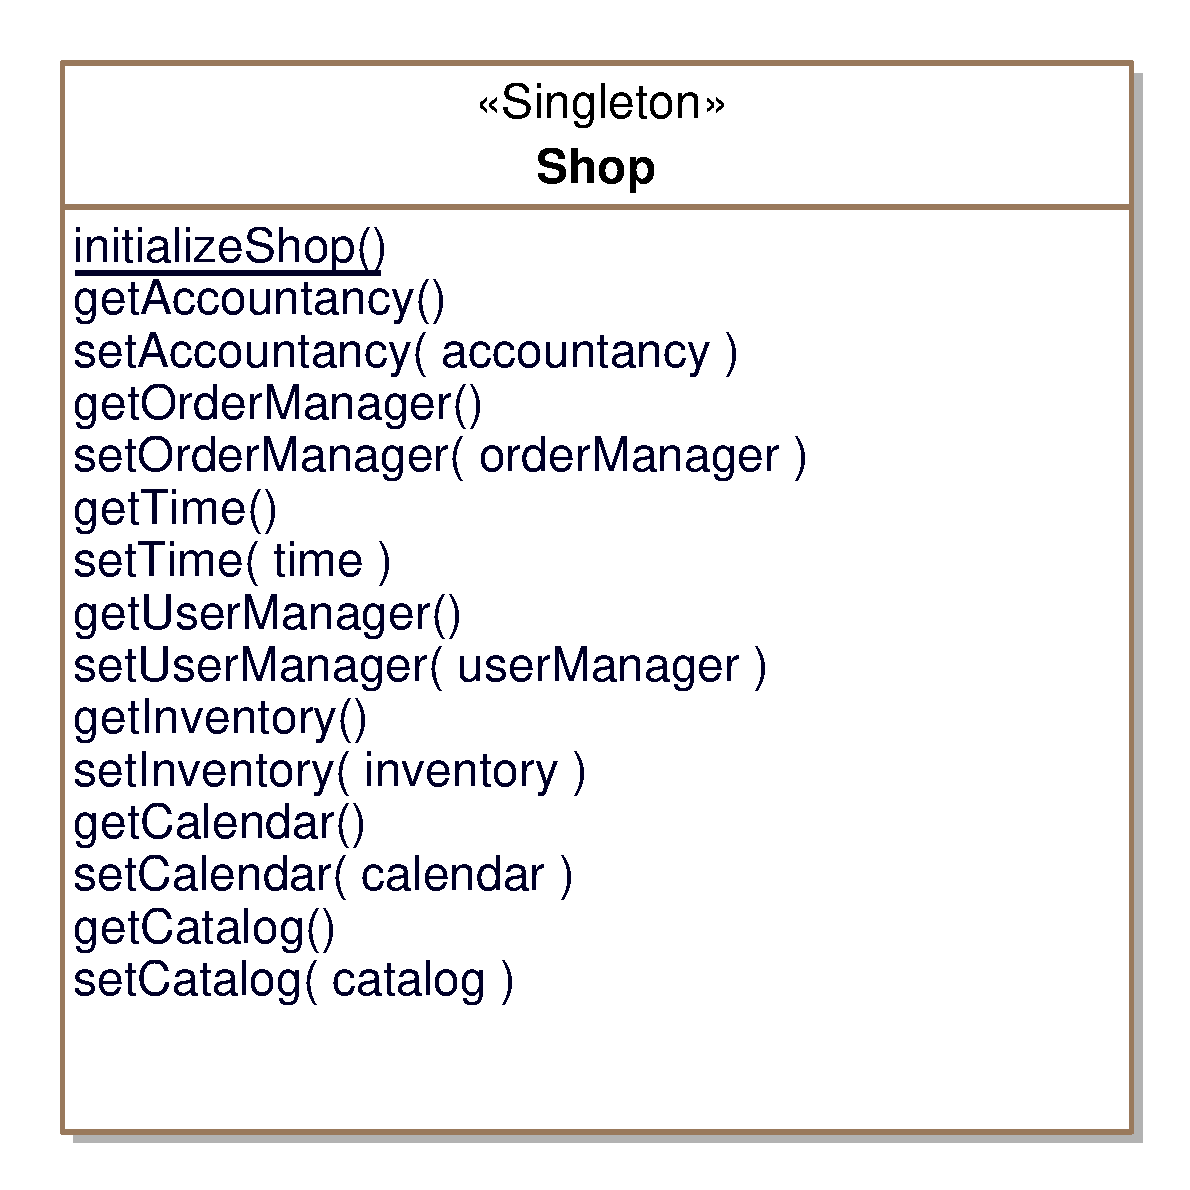
\includegraphics[width=1.0\textwidth]{images/Shop_Overview.eps}
	\label{shop_overview}
	\caption{Shop - Class Overview}
\end{figure}

\subsection{\code{Shop} - Starting your SalesPoint-application}
Every salesman needs one \code{Shop} to have a basement to sell his goods to his customer, so the \code{Shop}-enumeration is the basis of every SalesPoint-application and they exist no 
instances of it. With the method \code{initializeShop()} it will be initialize all interfaces to the database. All of these interfaces are very important to work perfectly with SalesPoint,
there are
\begin{itemize}
\item \code{UserManager}: Main-part of the user-package to manage \code{User}s and is used to log on and off them from the system.
\item \code{Calendar}: Main-part of the calendar-package to persist and manage \code{CalendarEntry}s.
\item \code{Catalog}: Persisting, updating and presenting \code{ProductType}s.
\item \code{Inventory}: Persisting, managing and storing \code{Product}s.
\item \code{OrderManager}: Main-part of corder-package to persist, update and remove {OrderEntry}s.
\end{itemize}
Also you can set these interfaces manually. Look at the uml-diagram above the text. You find a set-method for each interface.\\ If you want to know the updating time of your shop, you can get 
it or you can set the time to any point of time.
